\section{Tutorial}
\subsection{Creación del Proyecto}
\begin{figure}[ht]
  \centering
  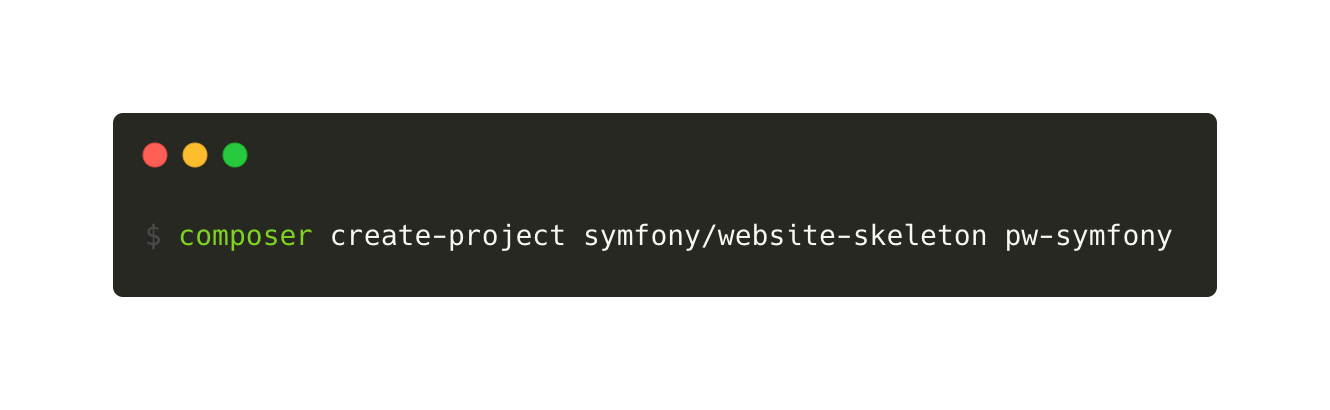
\includegraphics[width=\textwidth]{../assets/composer_create_project.png}
  \caption{Nuevo proyecto symfony con el cli}
  \label{fig:composer_create_project}
\end{figure}

Una vez creado el proyecto podemos utilizar el sevirdor intregrado en y utilizar el siguiente comando:

\begin{figure}[ht]
  \centering
  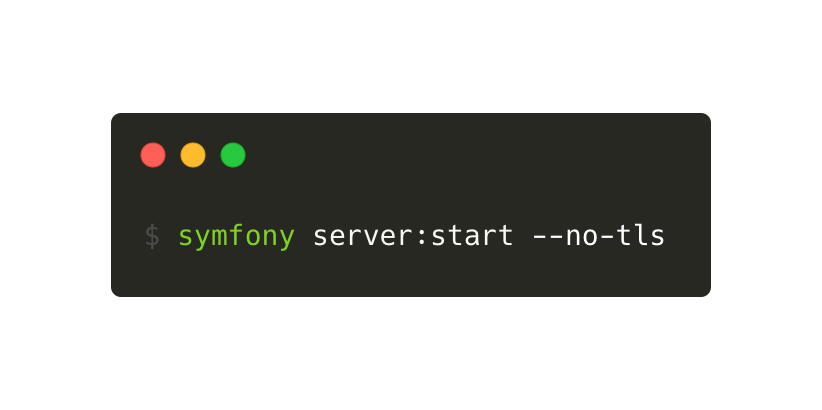
\includegraphics[width=\textwidth]{../assets/symfony_server_start.png}
  \caption{Iniciar el servidor integrado de symfony}
  \label{fig:symfony_server_start}
\end{figure}

\clearpage
Tambien podemos utilizar un servirdor apache, para que funcione bien podemos instalar el siguiente paquete:

\begin{figure}[ht]
  \centering
  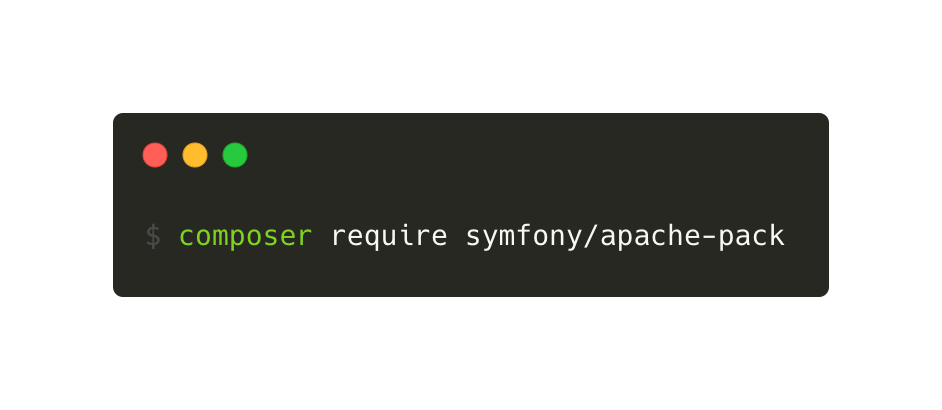
\includegraphics[width=\textwidth]{../assets/composer_apache.png}
  \caption{La forma más facil de configurar apache}
  \label{fig:composer_apache}
\end{figure}

Si todo funciona al abrir la siguiente url \href{http://localhost:8000}{http://localhost:8000} nos deberia aparecer la siguente pagina:

\begin{figure}[ht]
  \centering
  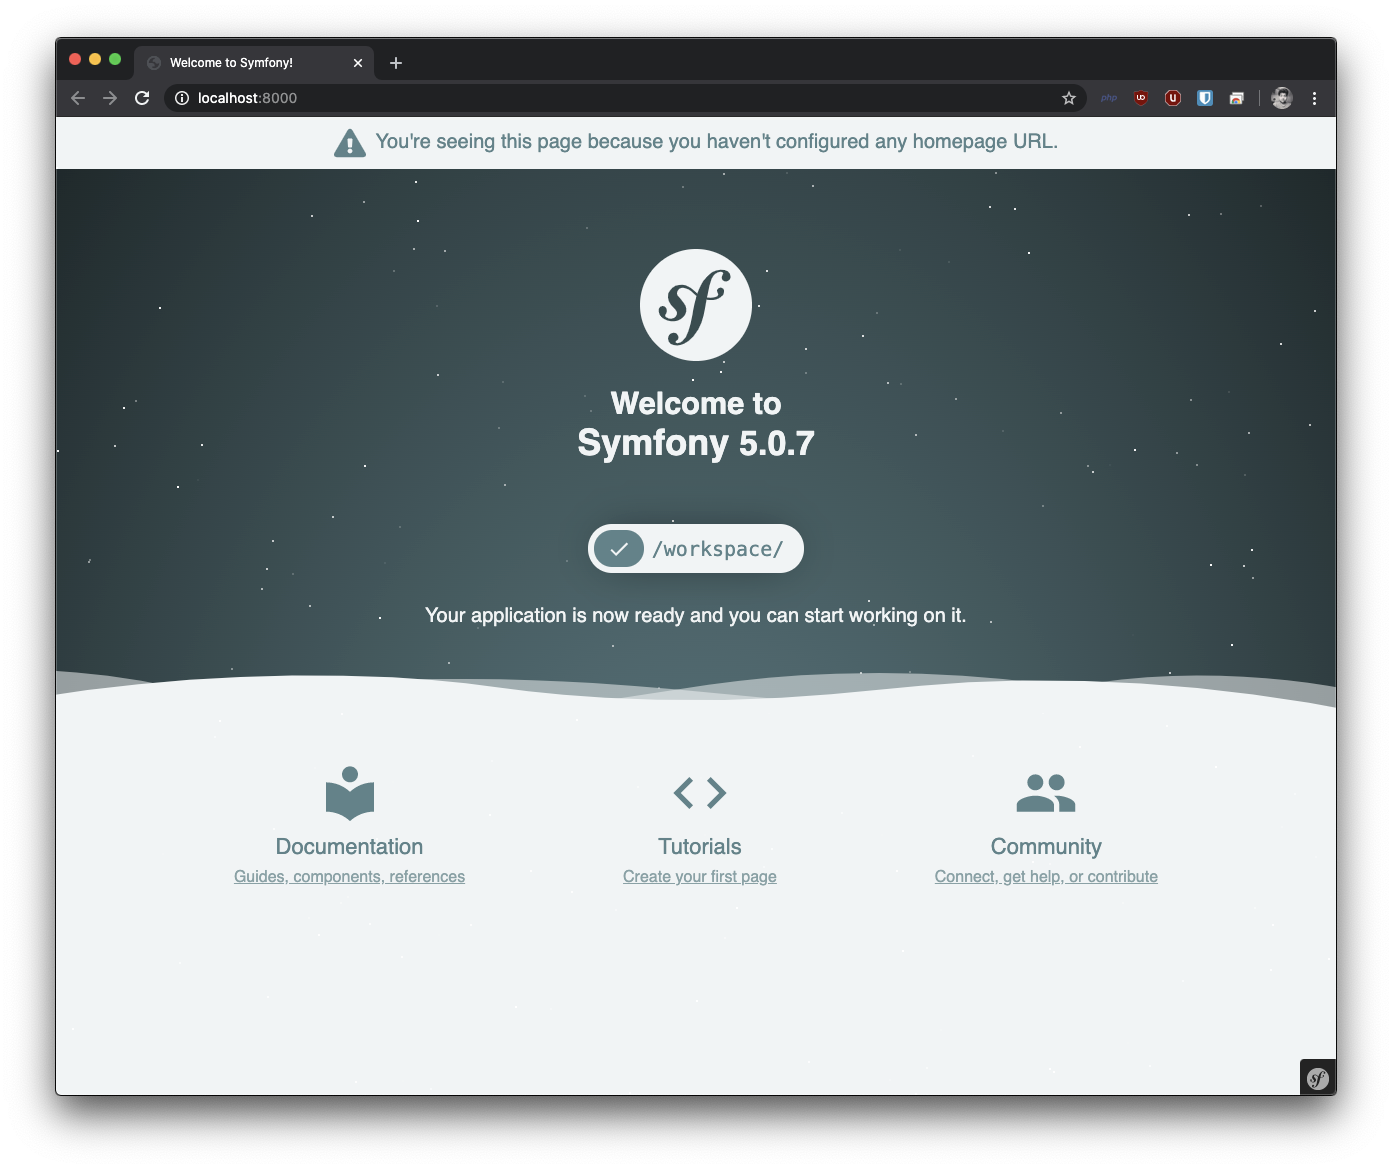
\includegraphics[width=0.7\textwidth]{../assets/symfony_main.png}
  \caption{Pagina principal symfony}
  \label{fig:symfony_main}
\end{figure}
\clearpage
\subsection{Configurando la base de datos}
Para que symfony pueda conectarse con nuestra base de datos debemos editar el fichero \texttt{.env} para modificar la varible \texttt{DATABASE\_URL}
\begin{figure}[ht]
  \centering
  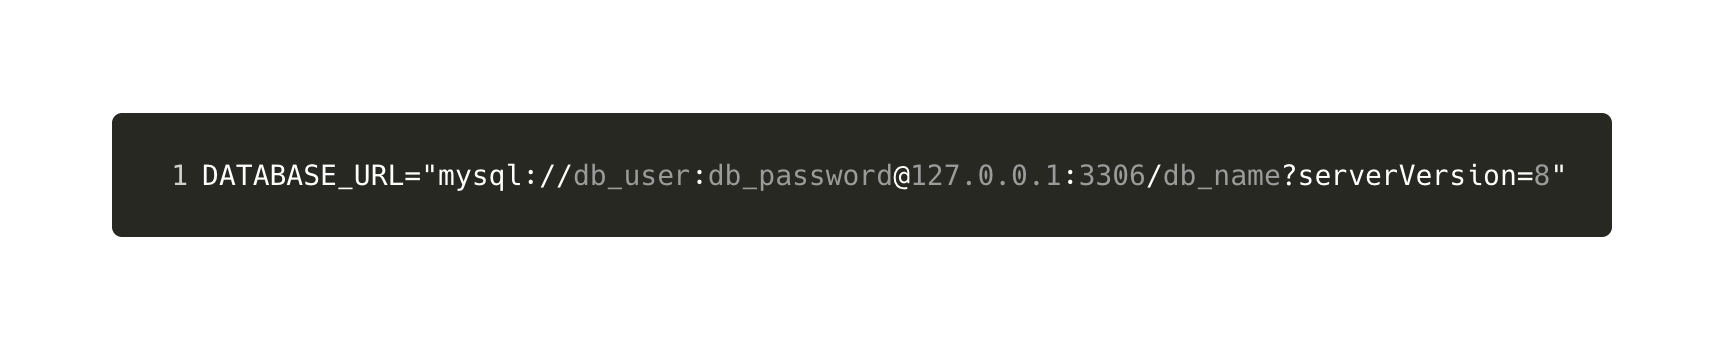
\includegraphics[width=\textwidth]{../assets/symfony_dot_env.png}
  \caption{Pagina principal symfony}
  \label{fig:symfony_dot_env}
\end{figure}

Las siguentes varible se pueden modificar acorde a nuestro caso de uso:

\begin{center}
  \begin{minipage}{0.4\textwidth}
    \begin{itemize}
      \item[mysql] Driver utilizando
      \item[db\_user] Nombre de usuario
      \item[db\_password] Contraseña del usuario
      \item[127.0.0.1] Host de la base de datos
      \item[3306] Puerto de la base de datos
      \item[serverVersion] Version de base de datos
    \end{itemize}
  \end{minipage}
\end{center}

Si antes no hemos creado nuestra base de datos podemos utilizar el siguente comando:
\begin{figure}[ht]
  \centering
  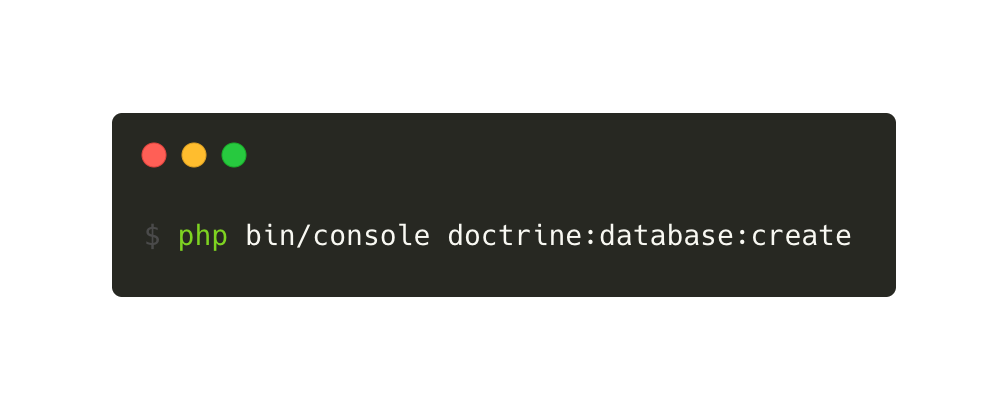
\includegraphics[width=\textwidth]{../assets/create_db.png}
  \caption{Crear base de datos}
  \label{fig:create_db}
\end{figure}
\clearpage
\subsection{Creando las Entidades}

Para crear una entididad debemos utilizar el siguiente comando:

\begin{figure}[ht]
  \centering
  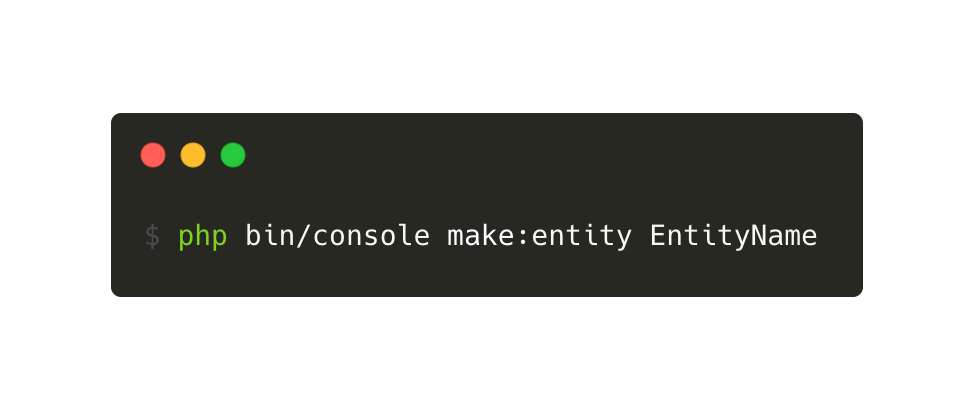
\includegraphics[width=\textwidth]{../assets/make_entity.png}
  \caption{Comando para crear una entididad}
  \label{fig:make_entity}
\end{figure}

En nuestro caso vamos a crear la entididad \texttt{Article} con las siguientes propiedades:

\begin{figure}[ht]
  \centering
  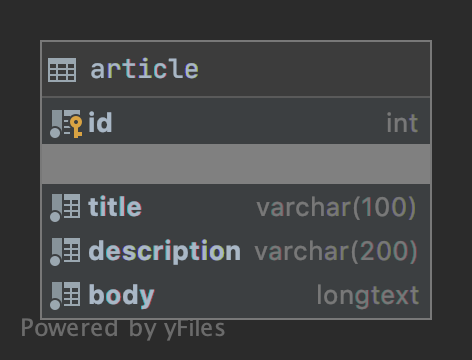
\includegraphics[width=0.4\textwidth]{../assets/article_sql.png}
  \caption{Entididad Article}
  \label{fig:article_sql}
\end{figure}

\begin{figure}[ht]
  \centering
  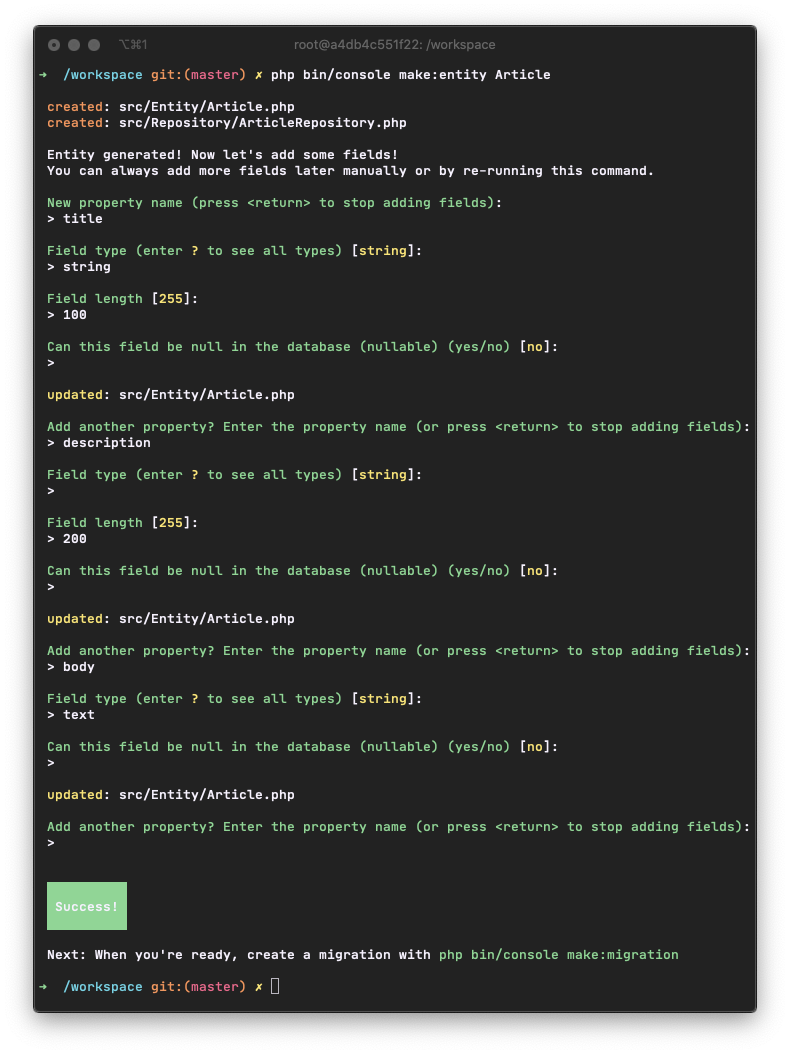
\includegraphics[width=\textwidth]{../assets/creation_article_entity.png}
  \caption{Creacion de la entidad \texttt{Article}}
  \label{fig:creation_article_entity}
\end{figure}
\clearpage

Como se puede observar en la \href{fig:creation_article_entity}{Figura anterior} el comando nos ira preguntado por la propiedades que deseamos añadir.

Una vez creada la entidad debemos hacer la migraciones ejecutando el siguiente comando:

\begin{figure}[ht]
  \centering
  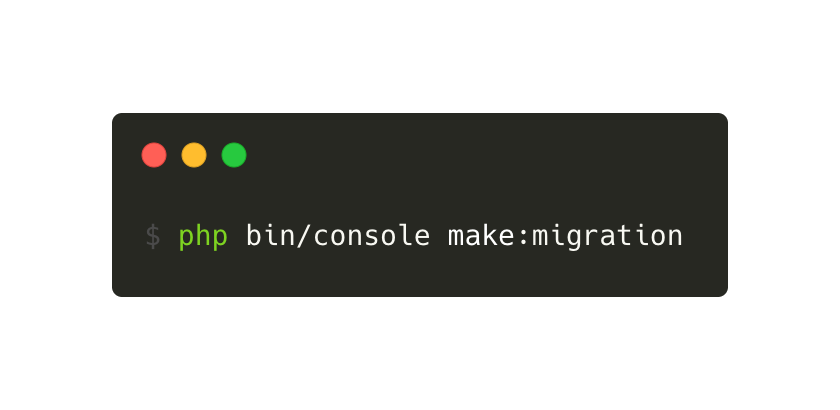
\includegraphics[width=\textwidth]{../assets/make_migration.png}
  \caption{Creando la migraciones}
  \label{fig:make_migration}
\end{figure}

Finalmente debemos aplicar la migraciones a nuestra base de datos ejecutando el siguiente comando:

\begin{figure}[ht]
  \centering
  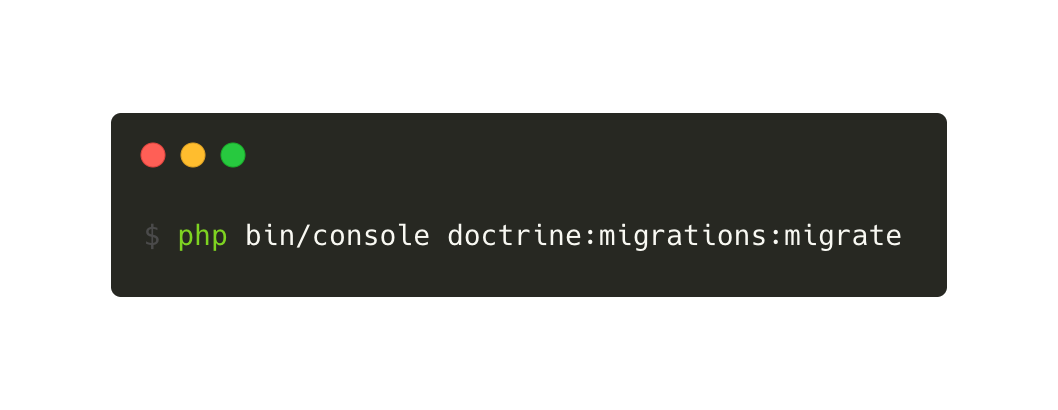
\includegraphics[width=\textwidth]{../assets/apply_migration.png}
  \caption{Aplicando las migraciones}
  \label{fig:apply_migration}
\end{figure}
\clearpage
\subsection{Creación de controlador y vistas de Artículo}

Para crear un controlador debemos utilizar el siguiente comando:

\begin{figure}[ht]
  \centering
  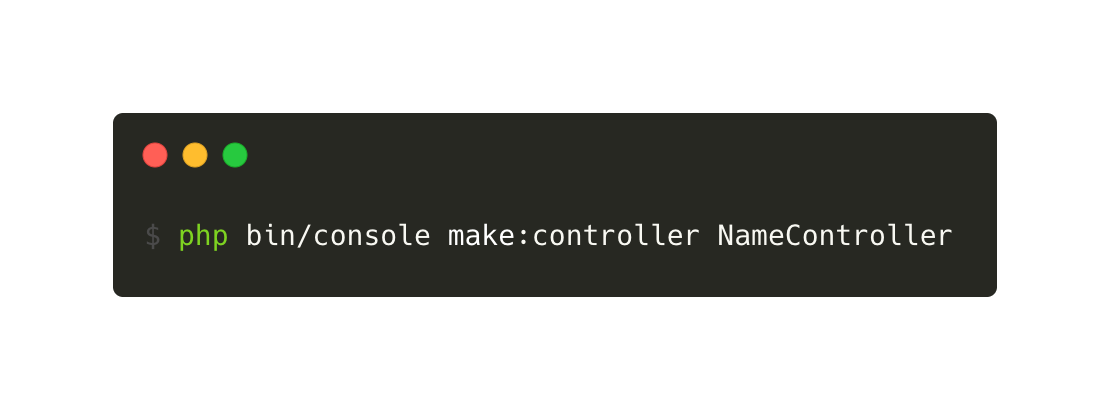
\includegraphics[width=\textwidth]{../assets/make_controller.png}
  \caption{Aplicando las migraciones}
  \label{fig:make_controller}
\end{figure}

Nos debe de crear los siguientes ficheros:


\begin{center}
  \begin{minipage}{0.4\textwidth}
    \begin{itemize}
      \item[\texttt{\textbf{src/Controller/ArticleController.php}}] Nuestro controlador.
      \item[\texttt{\textbf{templates/article/index.html.twig}}] Template por defecto.
    \end{itemize}
  \end{minipage}
\end{center}

A continuación vamos a \texttt{src/Controller/ArticleController.php}, y ahí tendremos el código de nuestro controlador de \textit{Articles}. Pasamos a dotarle de funcionalidad, como la de mostrar todos los artículos que tenemos en BD, para ello modificamos la función \texttt{index} añadiéndole lo siguiente:

\begin{figure}[ht]
  \centering
  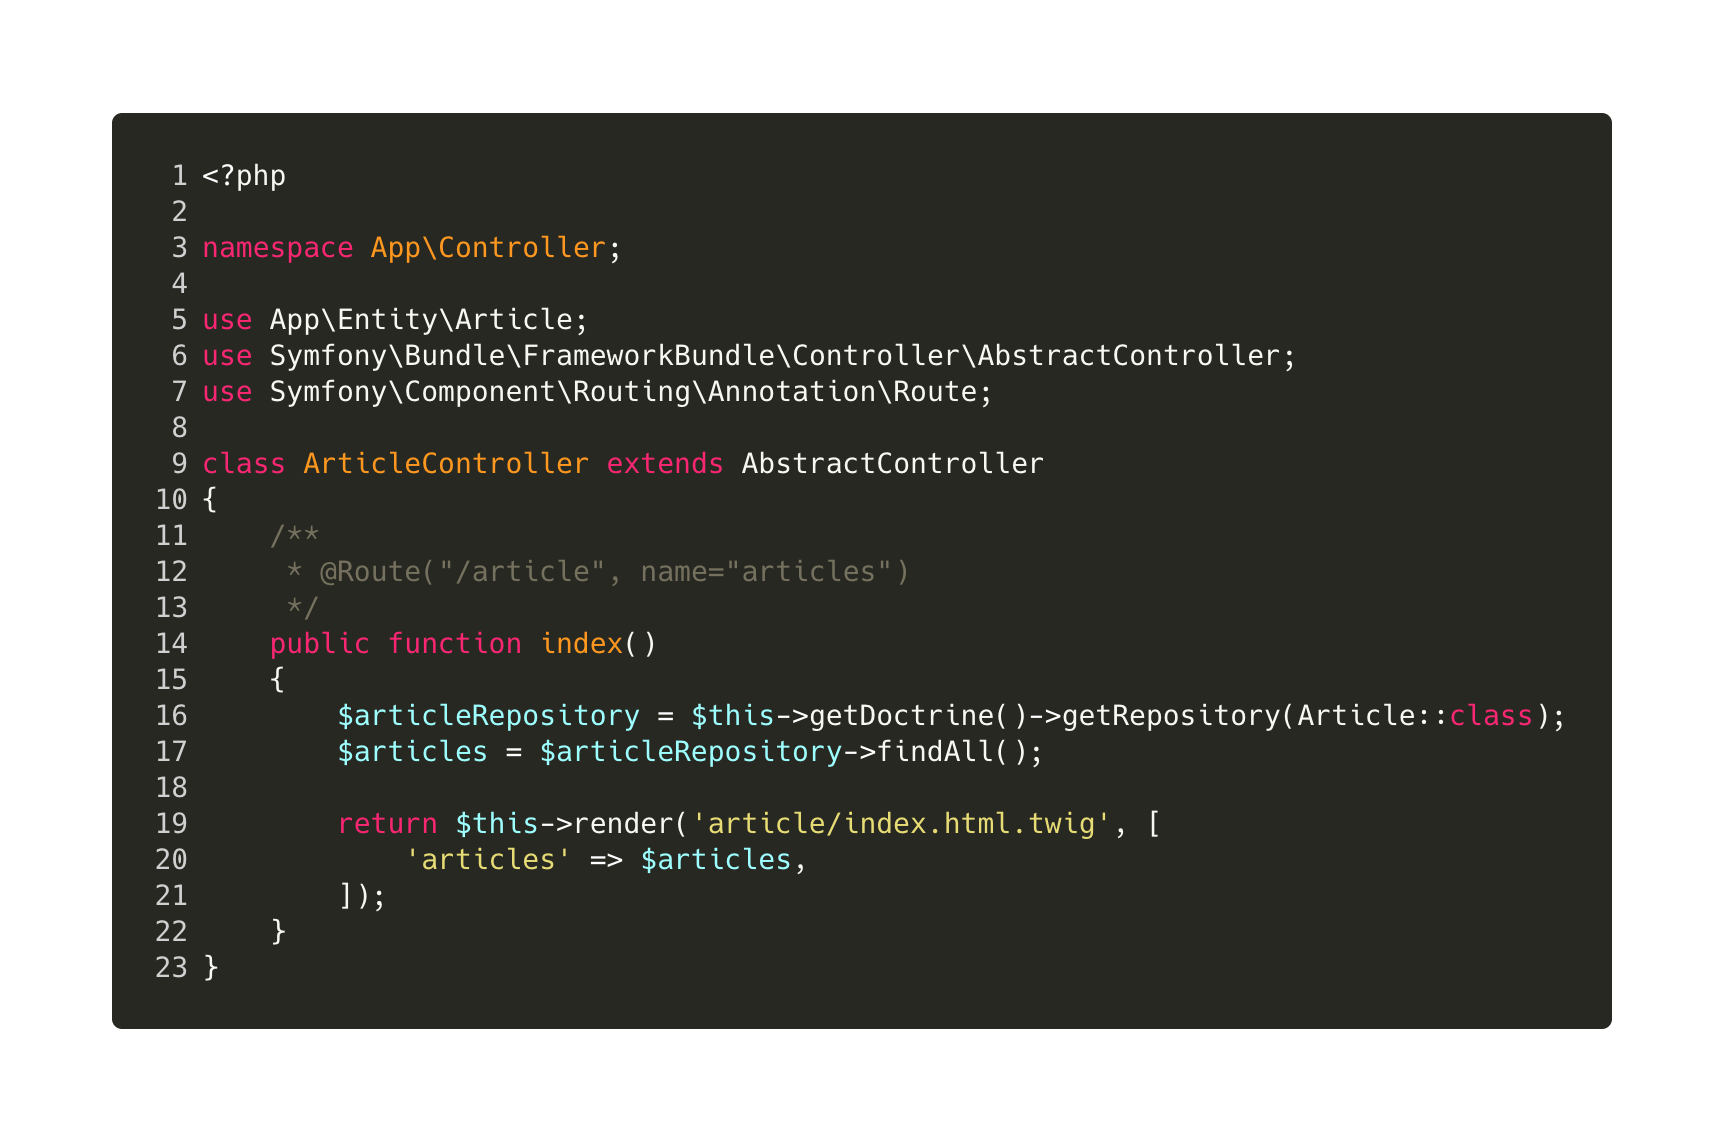
\includegraphics[width=\textwidth]{../assets/article_index.png}
  \caption{\texttt{ArticleController.php}}
  \label{fig:article_index}
\end{figure}

En la variable \texttt{\$articulosRepository} se guardará un objeto del manejador de la entidad de Doctrine, el cual es el objeto más importante en Doctrine, ya que es el responsable de guardar y obtener objetos de la base de datos.

En la variable \texttt{\$articles} se guardarán todos los artículos que se encuentren en la base de datos, y luego con el return \texttt{\$this->render()}, vamos a la vista index.\footnote{La vista plantilla ya viene creada por defecto en templates/base.html.twig y la carpeta de las vistas de Articulos también se crea sola al crear la entidad.}.

Así mismo crearemos un método llamado \texttt{show} en el controlador para mandar a una nueva vista llamada \texttt{article.html.twig} los datos de un artículo a partir de un \texttt{id}, que contendrá lo siguiente:

\begin{figure}[ht]
  \centering
  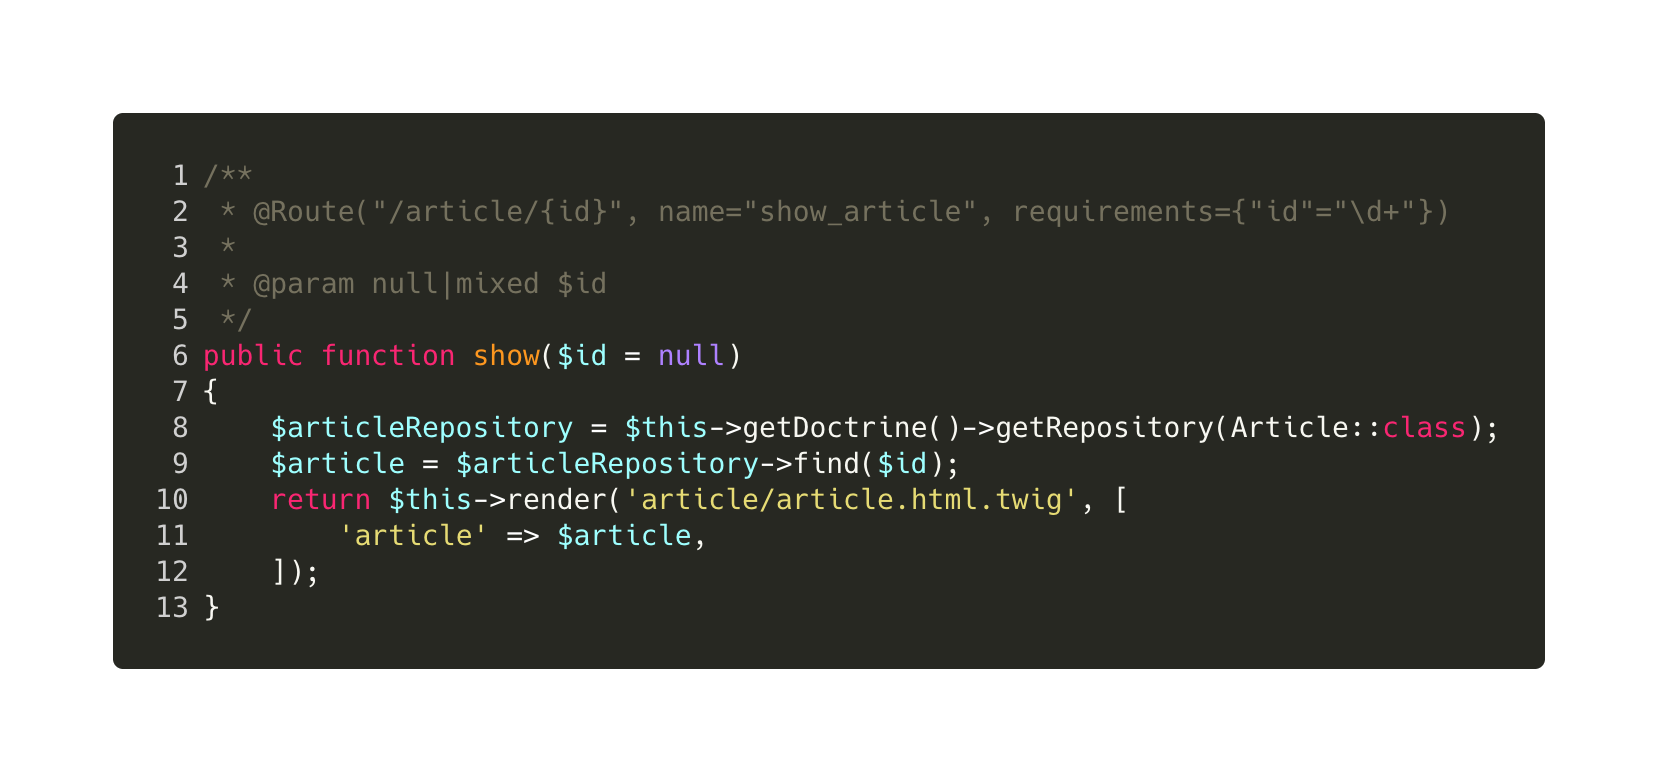
\includegraphics[width=\textwidth]{../assets/article_show.png}
  \caption{\texttt{\textbf{ArticleController::show}}}
  \label{fig:article_show}
\end{figure}

Tambien debemos editar la vista \texttt{\textbf{templates/article/index.html.twig}} con el siguente codigo:

\begin{figure}[ht]
  \centering
  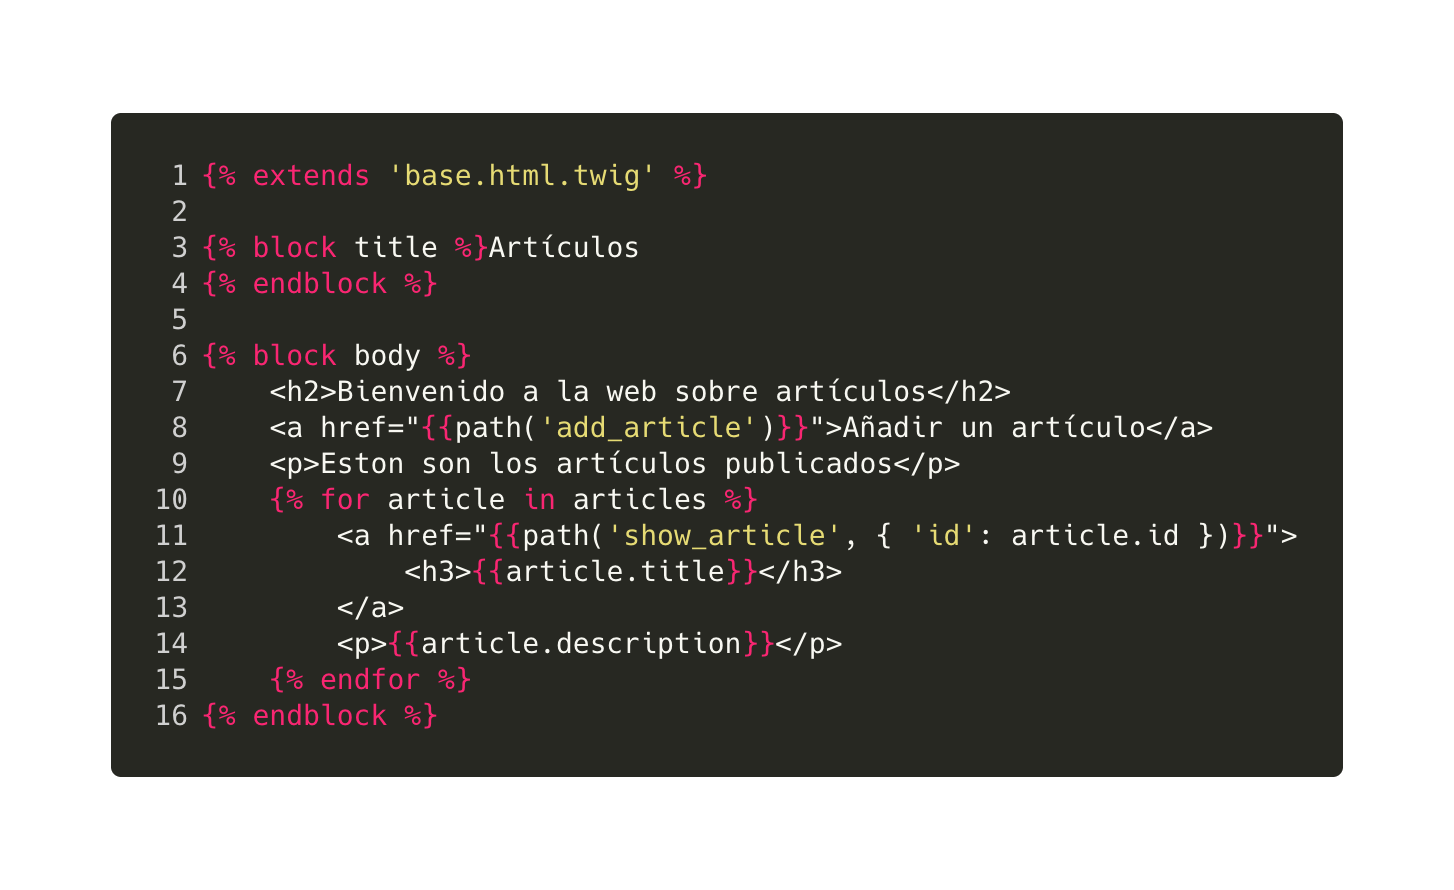
\includegraphics[width=\textwidth]{../assets/article_index_twig.png}
  \caption{Vista \texttt{\textbf{templates/article/index.html.twig}}}
  \label{fig:article_index_twig}
\end{figure}

\clearpage
Por ultimo debemos crear la vista \texttt{\textbf{templates/article/article.html.twig}} con el siguiente cotenido:

\begin{figure}[ht]
  \centering
  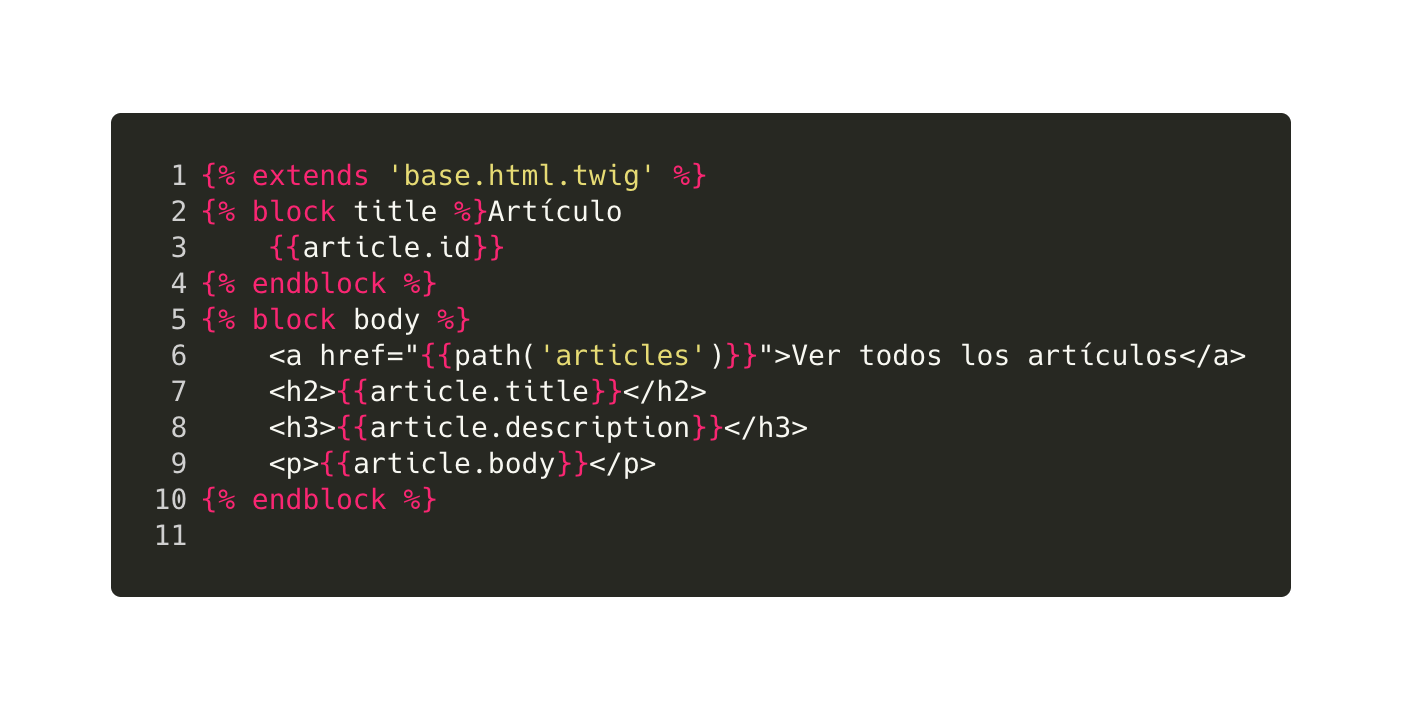
\includegraphics[width=\textwidth]{../assets/article_article.png}
  \caption{Vista \texttt{\textbf{templates/article/article.html.twig}}}
  \label{fig:article_article}
\end{figure}

\subsection{Creación de Formularios}

Para crear un formulario utilizaremos el siguiente comando:

\begin{figure}[ht]
  \centering
  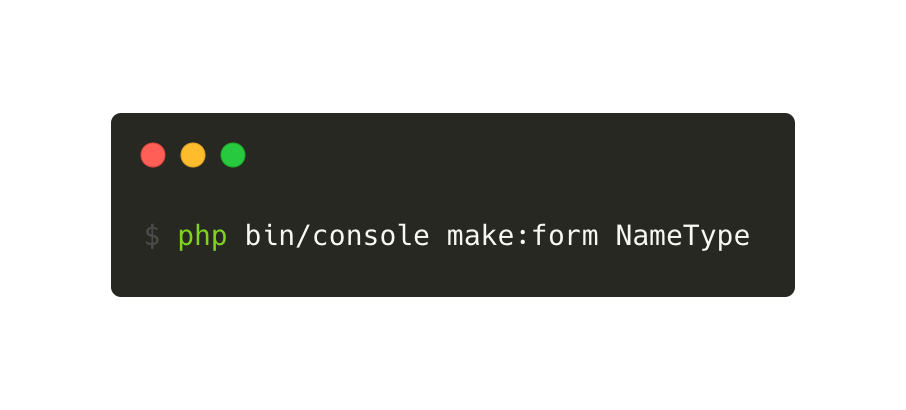
\includegraphics[width=\textwidth]{../assets/make_form.png}
  \caption{Comando para crear un formulario}
  \label{fig:make_form}
\end{figure}

\clearpage
Este comando nos generara el fichero \texttt{\textbf{src/Form/ArticleType.php}}, al que debemos editar con el siguiente código:

\begin{figure}[ht]
  \centering
  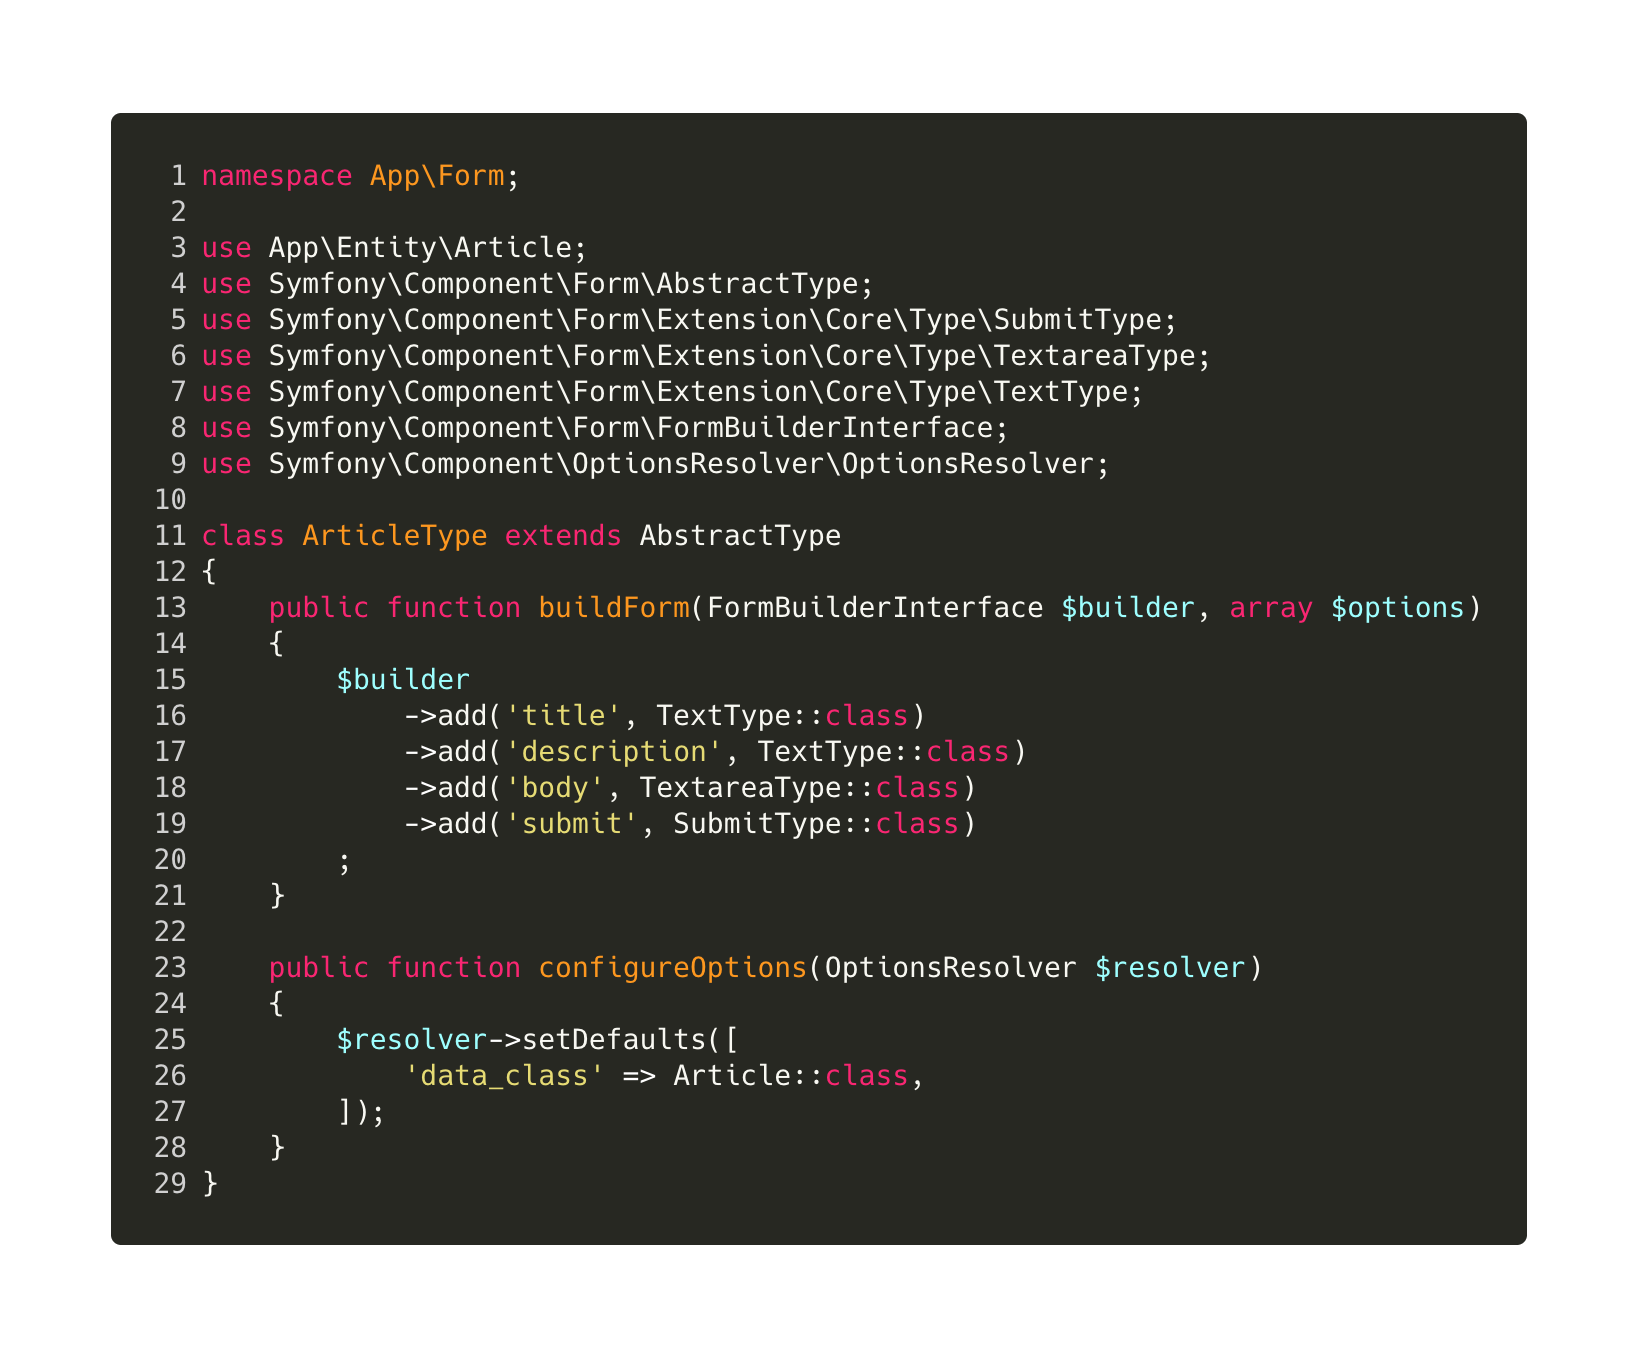
\includegraphics[width=\textwidth]{../assets/article_type.png}
  \caption{\texttt{\textbf{ArticleType}}}
  \label{fig:article_type}
\end{figure}

Después de haber creado el formulario, pasamos a crear la función de crear un nuevo artículo, y su vista correspondiente.
\clearpage
A la función la llamaremos \texttt{create}, su código será el siguiente:
\begin{figure}[ht]
  \centering
  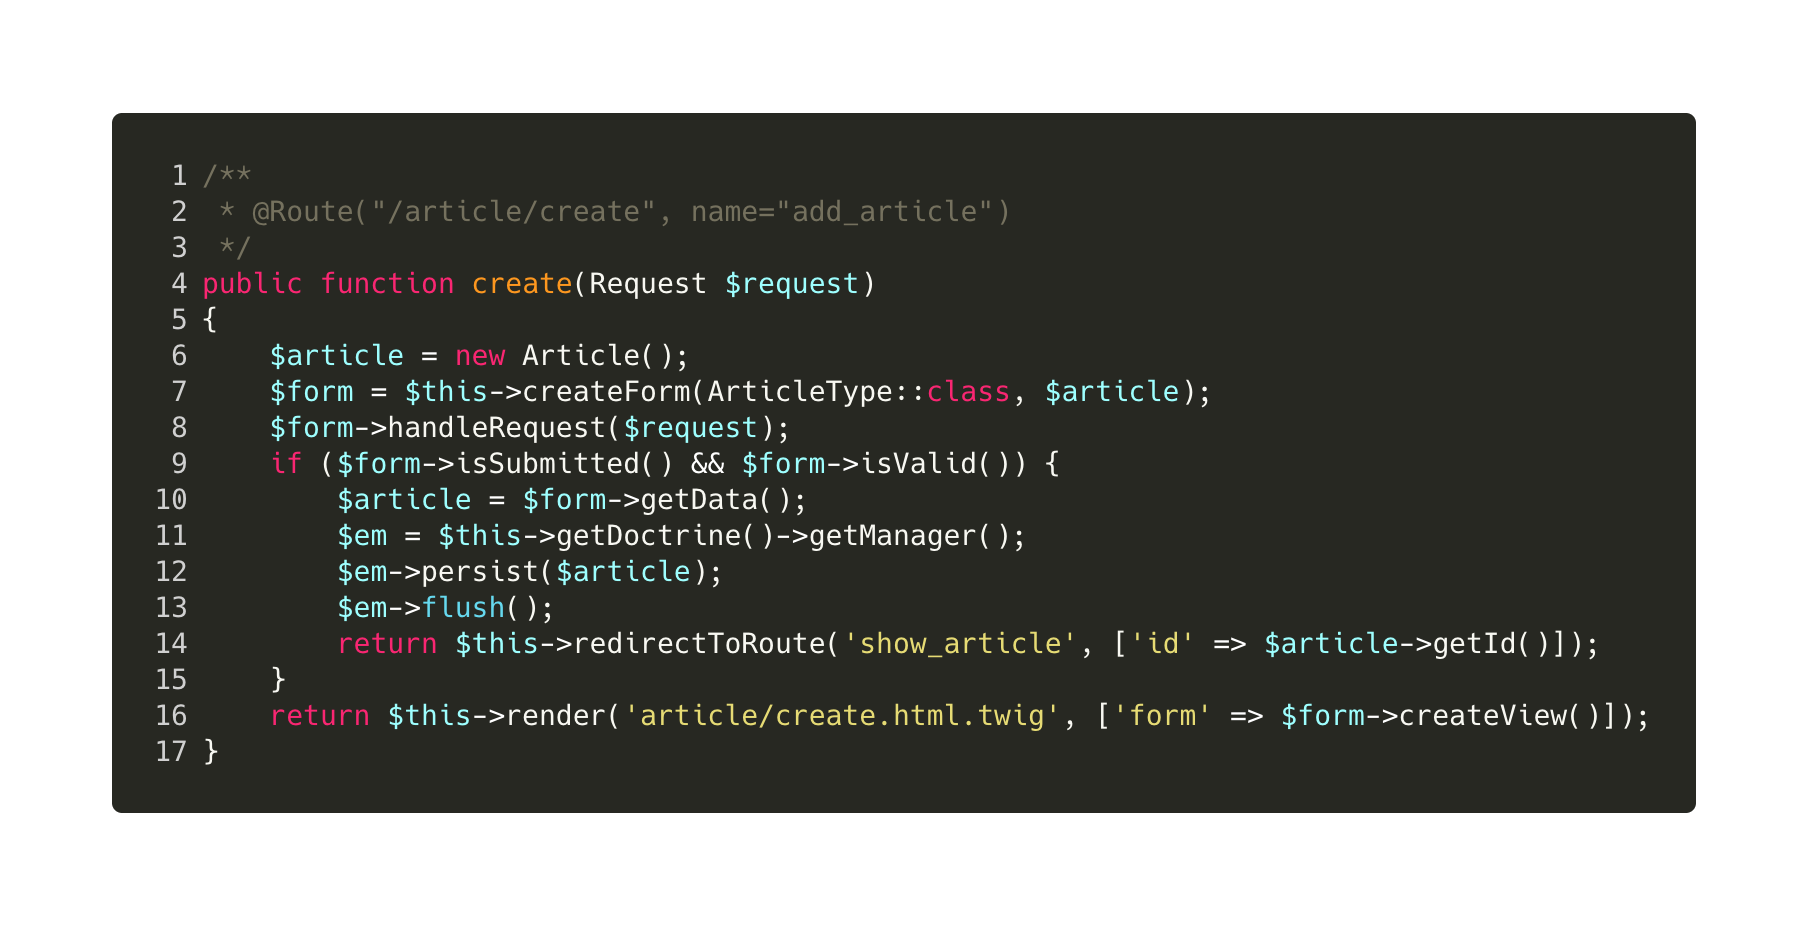
\includegraphics[width=\textwidth]{../assets/article_create_form.png}
  \caption{\texttt{\textbf{ArticleController::create}}}
  \label{fig:article_create_form}
\end{figure}

El codigo de la vista \texttt{\textbf{templates/article/create.html.twig}} es el siguente:

\begin{figure}[ht]
  \centering
  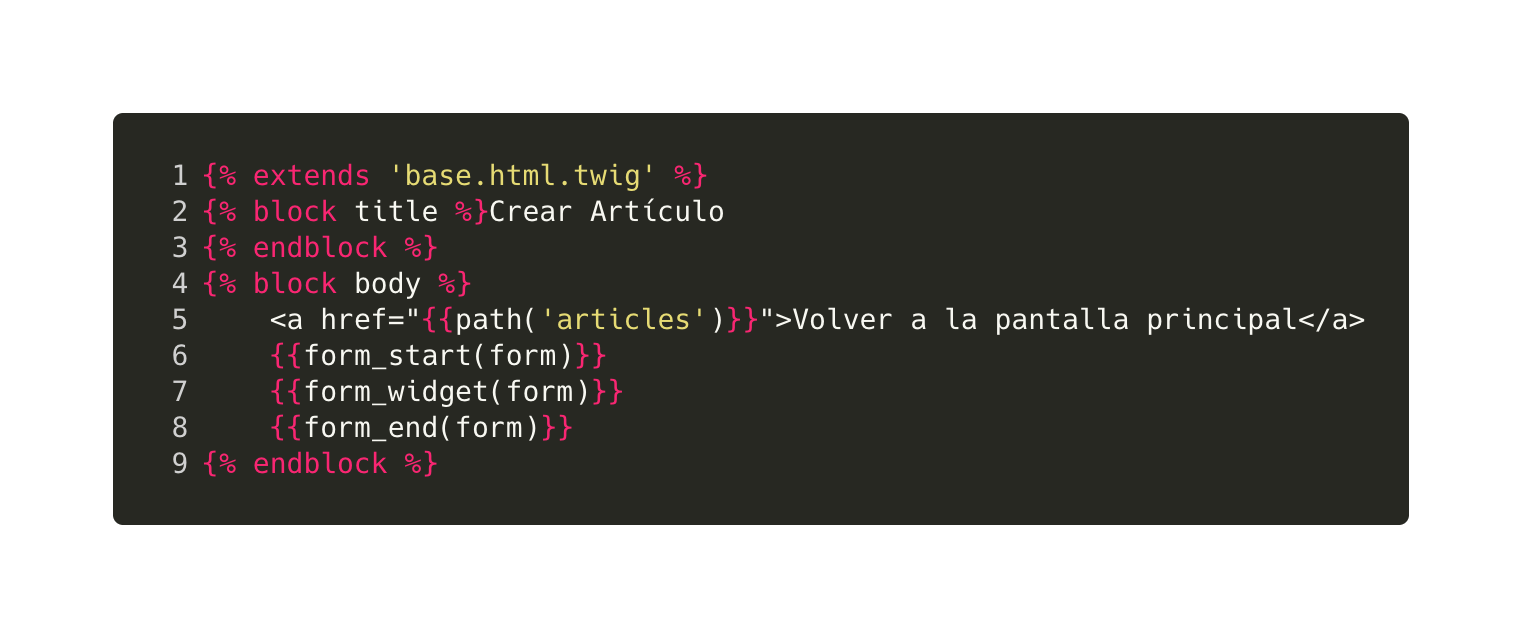
\includegraphics[width=\textwidth]{../assets/form_article_twig.png}
  \caption{Vista \texttt{\textbf{templates/article/create.html.twig}}}
  \label{fig:form_article_twig}
\end{figure}

\clearpage
Ahora si vamos a \texttt{http://localhost:8888/article} veremos la siguente vista:

\begin{figure}[ht]
  \centering
  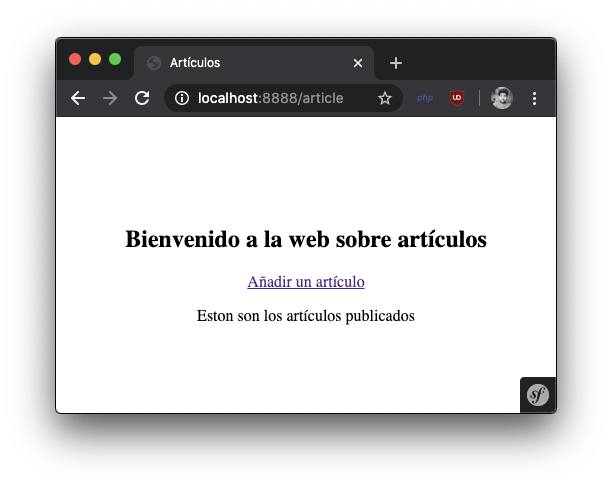
\includegraphics[width=\textwidth]{../assets/articles_render.png}
  \caption{Ruta \texttt{\textbf{article}}}
  \label{fig:articles_render}
\end{figure}

\clearpage
Si le damos a \textit{Añadir un artículo}, nos mandará la vista del \href{fig:article_create_form}{formulario} que hemos creado para crear nuestros artículos.

\begin{figure}[ht]
  \centering
  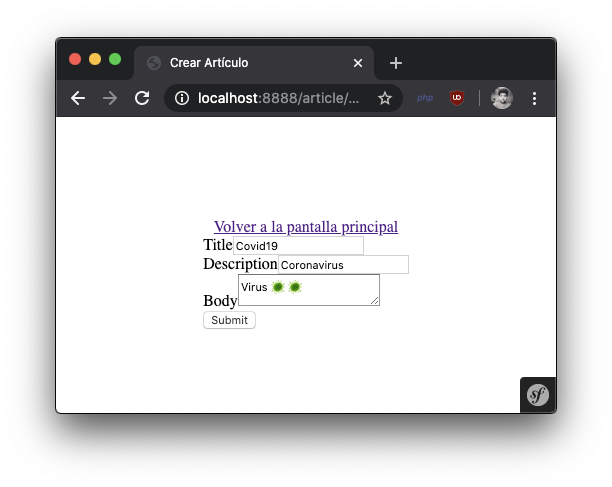
\includegraphics[width=\textwidth]{../assets/article_form_render.png}
  \caption{Ruta \texttt{\textbf{article/create}}}
  \label{fig:article_form_render}
\end{figure}

\clearpage
Para probar que funciona añadiremos los datos de un artículo de ejemplo y veremos que al hacer \texttt{submit} nos mandará a la vista de este artículo en concreto.

\begin{figure}[ht]
  \centering
  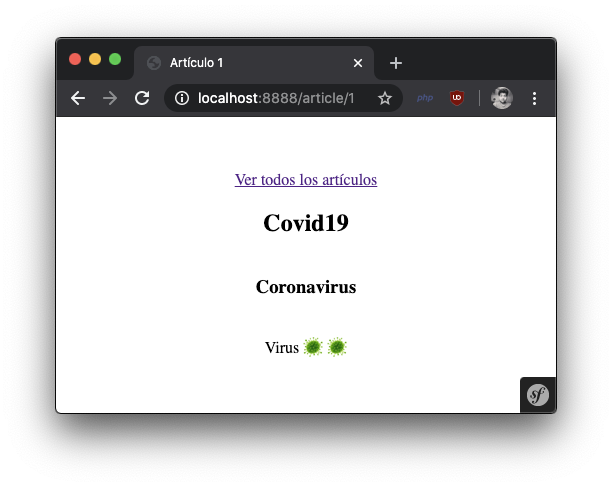
\includegraphics[width=\textwidth]{../assets/article_render.png}
  \caption{Ruta \texttt{\textbf{article/1}}}
  \label{fig:article_render}
\end{figure}

